
\section{Premier barnak}
\subsection{Coucou}
Sacristi de Jésus de\footnote{Saint-cimonaque de colon de sacréfice de tabarslaque de saintes fesses de cibouleau de purée.} plâtre de boswell de saintes fesses de sacrament de crucifix (\rref[Figure]{fig:pieux}) de mangeux d'marde (\rref[Table]{tab:my_label2}) de baptême de maudite marde de patente à gosse de colon de marde de câline de cochonnerie d'ostie de torvisse de géritole d'étole de tabarnak de mosus de gériboire de batèche d'enfant d'chienne de calvaire de cossin de charrue de ciboire de purée de torrieux.

\begin{figure}[!h]
    \centering
    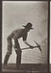
\includegraphics[width=.25\textwidth]{Introduction/stop1.png}
    \caption{Caption}
    \label{fig:antan}
\end{figure}

\subsection{Recoucou}
Sapristi de Jésus Marie Joseph de tabarnane de viarge de verrat de bâtard de calvinouche de cibole de cibouleau de saint-sacrament de charogne.

\begin{figure}[!h]
    \centering
    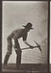
\includegraphics[width=.25\textwidth]{Introduction/stop1.png}
    \caption{Caption}
    \label{fig:pieux}
\end{figure}